

\chapter{测试框架设计}

在本部分中,将对整个测试框架的结构进行设计并描述该设计相对于已有的一些测试框架所具有的优势。

\section{总体设计}
对于整个测试框架,我们将其分为下面的几个部分:
\begin{itemize}
\item 内核编译系统。用于进行内核的编译工作,能够自动化的内核代码管理,以及内核编译任务管理,处理各种与编译相关的任务。
\item 测试管理系统。测试管理系统管理整个测试的流程以及进行测试任务的分配和测试机器的协调。
\end{itemize}

图\ref{fig:compile_test_relation}中表现了内核编译系统和测试管理系统之间的关系。测试管理系统会根据需要向内核编译系统提交内核编译任务,内核编译系统会将编译完成的内核提供给测试管理系统进行性能测试。

\begin{figure}[H]
\centering
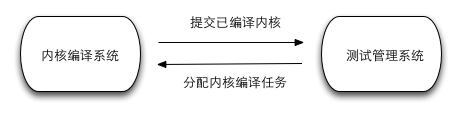
\includegraphics[width=12cm]{compile_test_relation}
\caption{内核编译系统与测试管理系统}
\label{fig:compile_test_relation}
\end{figure}

下面我们也将按照这两个系统对框架的设计进行介绍。

\subsection{内核编译系统}
内核的编译是一个非常耗时的过程,要想进行高效率的性能测试工作,那么高效率的内核编译是必不可少的。

图\ref{fig:compile_manage}中介绍的是内核编译系统的大致结构,整个内核编译系统可以分为两个部分:

\begin{itemize}
\item 编译管理服务器

编译管理服务器是整个内核编译系统的核心,编译管理服务器具有一下的职责:

\begin{enumerate}
\item 更新并合并各分支的内核源代码
\item 从测试管理系统获取编译任务
\item 将编译任务分配给每一个编译节点
\item 从编译节点获取编译完成的内核镜像
\item 向测试管理系统提供编译完成的内核
\end{enumerate}

\item 编译节点

每一个编译节点都是一台真实的计算机,并且运行的流程非常简单:
\begin{enumerate}
\item 编译节点空闲的时候会从编译管理服务器上面获取编译任务
\item 根据编译任务的要求开始编译内核
\item 将编译的记过保存在编译管理服务器上
\item 通知编译管理服务器已经完成相应的编译任务
\end{enumerate}

\end{itemize}


\begin{figure}[H]
\centering
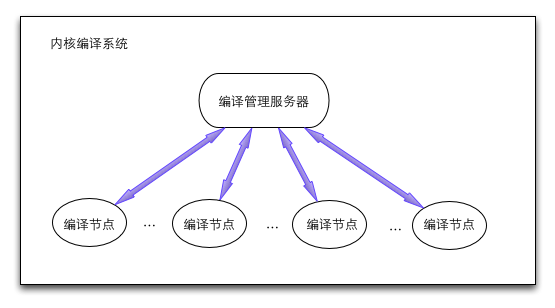
\includegraphics[width=12cm]{compile_manage}
\caption{内核编译系统结构}
\label{fig:compile_manage}
\end{figure}

\subsection{测试管理系统}

下面详细介绍一下测试管理系统的结构。

图\ref{fig:test_manage}是测试管理系统的结构图,和内核编译系统的结构类似,都由两个主要部分构成;
\begin{itemize}
\item 测试管理中心服务器 

相比于内核编译系统中的中心管理服务器,测试管理系统中的中心管理服务器具有更多的职责:

\begin{enumerate}
\item 生成性能测试任务
\item 根据性能测试任务给内核编译系统分配编译任务
\item 将性能测试任务分配给测试机
\item 处理和分析性能测试结果
\item 进行问题定位
\end{enumerate}

\item 测试机

对于测试机来说,需要完成的工作比较少,就是按照测试的流程执行相关的测试内容即可,和内核编译系统中的编译节点相比,比较大的一个区别是编译节点一般都是真实的计算机,而测试机既有可能是真实的计算机,也可能是一个普通的虚拟机,具体的测试流程将在下面的部分进行详细介绍。

\end{itemize}

\begin{figure}[H]
\centering
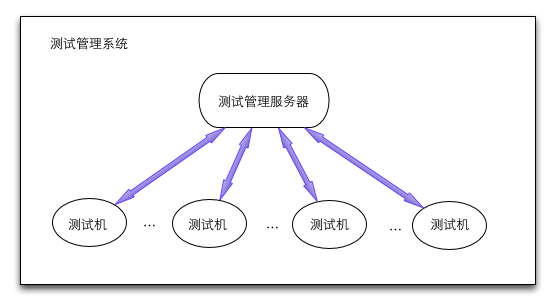
\includegraphics[width=12cm]{test_manage}
\caption{测试管理系统结构}
\label{fig:test_manage}
\end{figure}

下面详细介绍测试管理系统的处理流程。


\subsubsection{性能测试配置}

要进行性能测试,自然是需要有能够用于运行待测试内核的测试机,为了能够尽可能地提高性能测试效率,在我们的测试框架中,我们将使用具有Linux内核支持的KVM虚拟机来进行相关的测试工作。

在一台真实的计算机上,可以同时运行多台使用KVM技术的虚拟机,更为方便的是KVM虚拟机支持使用指定的内核和内存镜像文件来运行,这样,我们就可以不用花费大量的时间来进行内核镜像和内存镜像文件的打包,因此,使用虚拟机来进行内核的性能测试能够大大提高测试的效率。

另外,使用虚拟机还可以简化硬件的配置,因为虚拟机的硬件配置都是可以进行配置的,这样,可以使得我们的内核能够在更多的复杂硬件环境中运行,就更有可能发现内内核中存在的性能回退问题。

随着近几年来虚拟机技术的发展,越来越多的主机运营商也开始使用虚拟机来提供主机业务,因此虚拟机上的I/O性能也逐渐受到重视,因此使用虚拟机来进行内核性能测试是非常有必要的。

当然,我们的测试框架中所使用的不仅仅是虚拟机,毕竟虚拟机中的硬件模拟和真实硬件之间还是存在着比较大的区别,虚拟机测试是不能完全替代真机测试的,我们的测试也是能够在真机上轻松运行。

在我们的测试框架中,我们一般把每一次的性能测试称为一个测试任务,对于每一个测试任务,我们都用一个配置文件进行管理,这个配置文件将会对这一个测试任务进行全方位的配置,其中包括:
\begin{itemize}
\item 测试中需要运行的测试例程
\item 测试中需要启动的系统监视器
\item 测试机的硬件环境(包括硬盘和内存)
\end{itemize}

以上都是在进行测试之前就已经能够确定的一些测试参数,在完成一次性能测试任务之后,测试框架会向这个配置文件追加一些新的内容,其中包括:
\begin{itemize}
\item 进行测试的测试机信息
\item 该次测试所使用内核的commit ID
\item 该次测试所使用内核的分支及编译配置
\item 测试运行过程的时间和运行过程中的平均负载数据
\item 测试的当前状态
\item 测试结果的保存位置
\end{itemize}

在这里,我们需要在测试完成之后才记录下被测试内核的相关信息,这是由分配的机制导致的:在我们的框架中,性能测试内容和进行测试的内核的分配之间是互相分离的,测试机在获得一个需要进行测试的内核之后,再获取一个测试配置文件,结合两者进行测试,这样,测试系统能够在简单的实现下具有更高的效率,也能使得内核编译系统和测试管理系统之间配合得更加自然一些。

\subsubsection{测试机运行流程}

前面提到,在我们的测试框架中,进行测试的测试机既有可能是真实的计算机也有可能是KVM虚拟机,虽然测试机类型存在差异,但是在两种测试机上的运行的测试流程却是大致相同的。

\begin{figure}[H]
\centering
\includegraphics[width=8cm]{test_flow}
\caption{测试机运行流程}
\label{fig:test_flow}
\end{figure}

图\ref{fig:test_flow}中表示的就是在我们的测试框架中,所有测试机的运行流程,其中主要有下面的几个步骤:
\begin{enumerate}
\item 下载测试代码

从测试管理服务器上下载测试代码,这样,可以保证每次测试使用的测试代码都是最新的,这里的测试代码包括框架的运行代码

\item 挂载NFS

通过NFS挂载在测试管理服务器上的文件系统,并在相应的位置创建目录用于保存测试之后得到的测试数据

\item 配置环境

配置系统中相关的环境,其中包括配置结果保存的路径,挂载内核的调试文件系统


\item 进行测试

开始进行测试,在这一步中可以进一步细化为三个小的步骤:
\begin{enumerate}
\item 启动配置中要求的系统监视器
\item 执行测试例程
\item 停止系统监视器
\end{enumerate}

\item 保存测试结果

为了在测试中尽量减轻系统监视器对系统性能的影响,我们在测试进行的过程中的系统监视器输出都是保存在测试机本地的文件系统当中而不是测试管理服务器,因此,在测试完成之后,我们还需要将本地的测试结果通过NFS保存到测试管理服务器上

\item 通知任务完成

为了使得测试框架的效率最高,在我们的测试框架中使用的都是通信机制都是异步的,因此在测试结束后通知测试管理服务器,让测试管理服务器进行后面的处理

\item 收尾工作

在收尾工作中,我们将对两种情况分开处理:
\begin{itemize}
\item 如果测试机为虚拟机,那么直接执行reboot,由于在启动虚拟机的时候我们指定了不支持重新启动的选项,因此,在reboot之后kvm将会结束运行,从而开始进行下一次的测试
\item 如果测试机为真实的计算机,那么获取新的测试内核和执行任务,然后适用kexec来启动新的内核进行测试
\end{itemize}
\end{enumerate}


\subsubsection{问题自动定位}
在我们的测试框架中,我们将会对某个版本的内核进行测试,并使用一定的算法来处理这些测试数据,从中找到性能回退问题。

一旦找到性能回退的问题,我们会再次进行测试以确认这个回退问题,在确认性能回退问题之后,我们将会开始对造成这个性能回退问题的代码进行定位。

一般来说,性能回退问题往往是由某一次或者多次的修改造成的,我们的目标就是定位到造成性能回退问题的这一次修改。对于Linux内核来说,由于Linux内核开发的开放性,每天进入Linux内核代码树的代码不计其数,虽然其代码审查的制度比较严格,但是出现性能回退的问题的可能性还是存在的,而如果在出现问题之后,通过人工的方法,或者从问题版本简单地进行回溯测试,那么将会耗费大量的时间,所以使用计算机自动检测并采用比较好的查找算法可以大大提高性能回退问题的查找时间。

幸运的是,Linux内核源代码的管理使用的是git,git是一种非常高级的代码版本管理工具,它不仅可以进行代码版本的管理,还能高效并且准确地自动进行问题代码的定位。

在我们的测试框架中,就是使用了git的这一原生功能来进行错误代码的定位的,这一功能在git中被称为bisect,git中的bisect使用的查找算法是二分查找:指定一个好的版本和一个出现问题的版本,bisect每次都会从两个版本正中间的版本进行测试判断,这样就可以在$O(\log{n})$的复杂度内找到出现问题的版本。

其中,用于进行判断的方法是由用户提供的,所以我们的测试框架还必须提供这个用于判断性能回退的算法,这个算法将在后面的章节进行详细介绍。


\section{提升与优势}

我们新设计的框架相对于已有的一些测试框架和具有相似功能的框架相比具有很大的提升和更多的优势。

\begin{itemize}
\item 与LKP相比

\begin{enumerate}
\item 覆盖更多的开发分支,能够更早地发现潜在的性能回退
\item 具有更高的测试效率
\item 拥有更加全面和完善的数据处理和分析能力
\item 提供更加详细,更加丰富的测试结果报告
\item 尽可能充分利用已有的计算资源
\end{enumerate}

\item 与MMTests相比

\begin{enumerate}
\item 拥有更为完善和统一的数据处理流程
\item 拥有更全面的测试数据覆盖
\item 具有更完整的测试流程
\item 具有数据分析功能
\item 具有问题定位功能
\end{enumerate}

\end{itemize}